\subsection{Optimalizace s využitím náhradního modelu}\label{model-based}
V případech, kdy je vyčíslení účelové funkce v konkrétním bodě časově nebo výpočetně  náročné, je užitečné během optimalizace v nějaké formě využít náhradu účelové funkce. Definujeme náhradní model (anglicky \textit{surrogate model}) zkoumané úlohy jako úlohu
\begin{equation}
	\min_{\vec{x} \in \mathbf{\tilde{X}}} \tilde{f}(\vec{x}),
\end{equation}
kde
\begin{equation}
	\mathbf{\tilde{X}} = \big\{ \vec{x} \in \mathbf{D} \subseteq \mathbb{R}^n \ | \ \vec{\tilde{g}} (\vec{x}) \leq \vec{0} \wedge \vec{\tilde{h}} (\vec{x}) = \vec{0} \, \big\},
\end{equation}
přičemž funkce $ \tilde{f}, \vec{\tilde{g}}$ a $ \vec{\tilde{h}} $ mají podobný charakter, jako funkce $ f, \vec{g} $ a $ \vec{h}$ z původní úlohy. Charakter funkcí $ \tilde{f}, \vec{\tilde{g}}$ a $ \vec{\tilde{h}} $ je záměrně vymezen neurčitě - tento způsob definice odpovídá tomu, že po náhradním modelu nutně nepožadujeme, aby byl vhodným aproximativním modelem původní úlohy \cite{two-decades, BBO-textbook, Kramer2011}. Dobrý aproximativní model totiž nemusí být z hlediska optimalizace vhodnou náhradou, tato situace je znázorněna na obr. \ref{fig:surrogate}.

\begin{figure}[H]
	\centering
	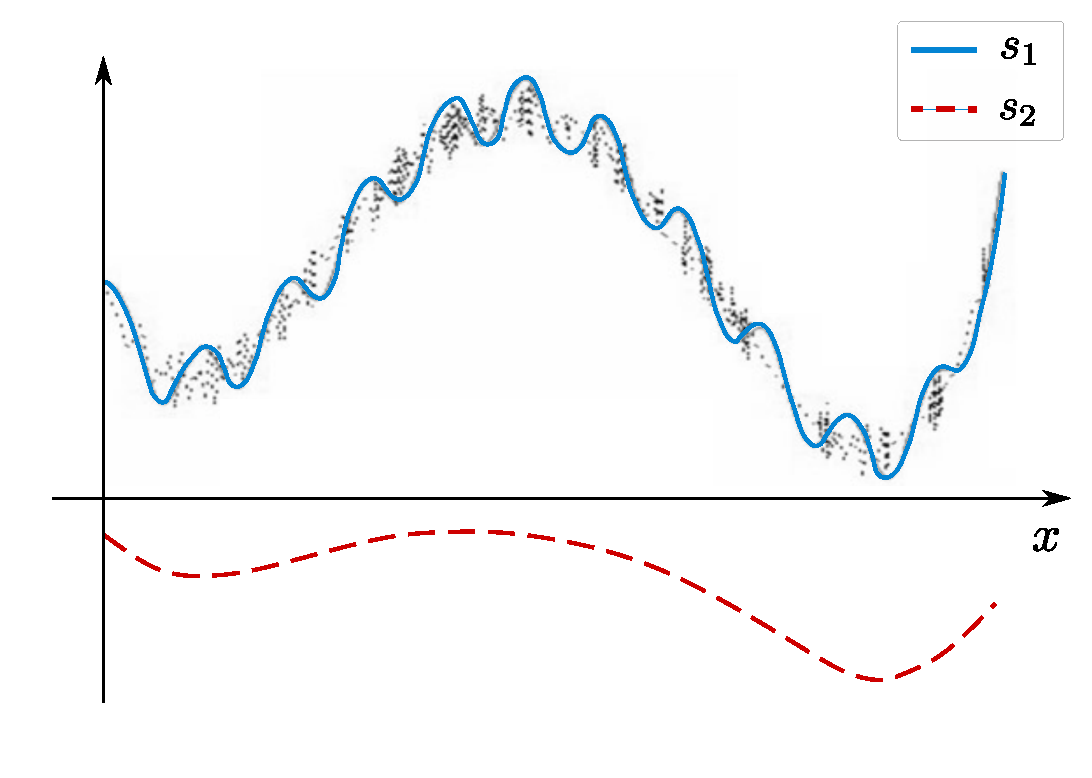
\includegraphics[width=0.6\textwidth]{figures/surrogate.pdf}
	\caption{Ilustrace dvou náhradních modelů $ s_1 $ a $ s_2 $. Černě jsou vyznačeny hodnoty účelové funkce vykazující šum. Použití náhradního modelu $ s_1 $ představuje volbu lepší z hlediska aproximace funkce, pro optimalizaci však tato volba vhodná není, jelikož $ s_1 $ obsahuje mnoho nežádoucích stacionárních bodů, které původní účelová funkce nemá. Na druhou stranu náhradní model $ s_1$ vhodně neaproximuje účelovou funkci ve smyslu funkčních hodnot, z hlediska optimalizace jde však o lepší volbu, jelikož stacionární body $ s_2$ se nacházejí na téměř shodných pozicích, jako je tomu u optimalizované účelové funkce.}
	\label{fig:surrogate}
\end{figure}

Využití náhradního modelu v rámci optimalizace je většinou dílčí částí jiné obecné optimalizační metody. Náhradní modely lze např. použít v rámci metod GPS a MADS popsaných v sekci \ref{direct-search}, kdy při vyčíslování účelové funkce v kroku průzkumu nejdříve vyčíslíme v těch samých bodech náhradní funkci $ \tilde{f} $, tyto hodnoty pak seřadíme, a již seřazenou množinu bodů použijeme k vyčíslení původní funkce $ f $. To nám umožní potenciálně výrazně zkrátit čas, který je potřebný k provedení kroku průzkumu, jelikož seřazením bodů zvýšíme pravděpodobnost, že úspěšně najdeme lepší odhad řešení již pro jeden z prvních zkoumaných bodů \cite{BBO-textbook}. Náhradní modely lze použít i v rámci jiných metod a urychlit tak jejich průběh, detailně je jejich použití rozebráno např. v \cite{two-decades, BBO-textbook}.